\documentclass[11pt]{beamer}
\usepackage{graphicx}
\graphicspath{ {./Images/} }
\setbeamertemplate{caption}[numbered]
\usepackage{caption}
\usepackage{float}
\usepackage{wasysym}
\usepackage{hyperref}
\usepackage{movie15}
%\usepackage[margin=1in]{geometry}
\usepackage{multirow}
\setbeamersize{text margin left=0.5cm,text margin right=0.5cm}
\usepackage{dirtytalk}
\usepackage{siunitx}
\usepackage{multicol}
\usepackage{listings}
\usepackage{color}
\usepackage{fancyvrb}
\usepackage{booktabs} % Allows the use of \toprule, \midrule and \bottomrule in tables
\definecolor{dkgreen}{rgb}{0,0.6,0}
\definecolor{gray}{rgb}{0.5,0.5,0.5}
\definecolor{mauve}{rgb}{0.58,0,0.82}
\lstset{
  language=Java,
  aboveskip=3mm,
  belowskip=3mm,
  showstringspaces=false,
  columns=flexible,
  basicstyle={\small\ttfamily},
  numbers=none,
  frame=single,
  numberstyle=\tiny\color{gray},
  keywordstyle=\color{blue},
  commentstyle=\color{dkgreen},
  stringstyle=\color{mauve},
  breaklines=true,
  breakatwhitespace=true,
  tabsize=3,
  fancyvrb=true,
}

% The following code is to pause within the align environment 
\makeatletter
\let\save@measuring@true\measuring@true
\def\measuring@true{%
  \save@measuring@true
  \def\beamer@sortzero##1{\beamer@ifnextcharospec{\beamer@sortzeroread{##1}}{}}%
  \def\beamer@sortzeroread##1<##2>{}%
  \def\beamer@finalnospec{}%
}
\makeatother

\mode<presentation> {
    \usetheme{Warsaw}
    % \setbeamertemplate{footline} % To remove the footer line in all slides uncomment this line
    \setbeamertemplate{footline}[page number] % To replace the footer line in all slides with a simple slide count uncomment this line
    % \setbeamertemplate{navigation symbols}{} % To remove the navigation symbols from the bottom of all slides uncomment this line    
    % \addtobeamertemplate{navigation symbols}{}{%
    %     \usebeamerfont{footline}%
    %     \usebeamercolor[fg]{footline}%
    %     \hspace{1em}%
    %     \insertframenumber/\inserttotalframenumber
        % }
    }
    
% macro for color
\definecolor{violet}{rgb}{0.54, 0.17, 0.89}
\newcommand{\red}[1]{\textcolor{red}{#1}}
\newcommand{\violet}[1]{\textcolor{violet}{#1}}
\newcommand{\green}[1]{\textcolor{green}{#1}}
\newcommand{\sol}{\textbf{Solution}: \pause \newline}

%----------------------------------------------------------------------------------------
%	TITLE PAGE
%----------------------------------------------------------------------------------------

\title[Chapter 06 Notes]{Math 130: Introduction to Programming \\ Chapter 06: A First Look at Classes \\ Lecture Notes}

\author{Jesús R. Pérez Cuarenta \\
\href{mailto:jperezcuarenta@swccd.edu}{jperezcuarenta@swccd.edu}
}

\date{} % Date, can be changed to a custom date

\begin{document}
% 
% The Splash Slide(s) are not part of any section
% 
% \section{}
%%%%%%%%%%%%%%%%%%%%%%%%%%%%%%%%%%%%%%%%%%%%%%%%%%%%%%%%%%%%%%%%%%%%%% 

\begin{frame}
  \maketitle
\end{frame}

\begin{frame}
\frametitle{Overview}
    % \begin{multicols}{2}
    \tableofcontents
    % \end{multicols}
\end{frame}

\section{Objects and Classes}
\subsection{Objects}
\begin{frame}{Objects}
    An object is a software component that exists in memory and serves a specific purpose in a program. \\ 
    \vspace{1em}
    An \red{object is created from a class} that contains code describing the object. \\ 
    \vspace{1em} 
    Think of a car's components: steering wheel, accelerator pedal, brake pedal, gear shifter, speedometer, engine, battery, radiator, and so on. 
\end{frame}

\begin{frame}{Objects}
    As an example, we can say that there exists a blueprint called Cars. \\
    \vspace{1em}
    Imagine one instance of the Cars blueprint to be a 1969 Pontiac GTO. We refer to this specific car model as an object. \\
    \vspace{1em}
    Similarly, the following can be thought of as other objects derived from the Cars blueprint: Tesla Model 3, Subaru WRX Impreza STI, Toyota Tacoma, Ford Ranger, etc.    
\end{frame}

\begin{frame}{Objects}
    In programming the blueprint doesn't exist in the physical world. \\ 
    \vspace{1em}
    In software, an object has two general capabilities: \\ 
    \vspace{1em}
    \begin{itemize}
        \item An object can \red{store data}. The data stored in an object are commonly called \red{fields}.
        \item An object can perform \red{operations}. The operations that an object can perform are called \red{methods}.
    \end{itemize}
\end{frame}

\begin{frame}{Objects}
    When a program needs the services of a particular type of object, it creates that object in memory, and then calls that object’s methods as necessary. \\ 
    \vspace{1em}
    Some examples we have seen already include: \\
    \vspace{1em}
    \begin{itemize}
        \item When reading input from a keyboard we can use a \textbf{Scanner} object.
        \item When generating random numbers we can use a \textbf{Random} object.
        \item When writing output to a file we can use a \textbf{PrintWriter} object.
    \end{itemize}
\end{frame}

\subsection{Classes}
\begin{frame}{Classes}
    Objects are very useful, but they don’t just magically appear in your program. \\ 
    \vspace{1em}
    Before a specific type of object can be used by a program, that object has to be created in memory. \\
    \vspace{1em}
    \red{Before an object can be created in memory, you must have a class for the object.} \\ 
    \vspace{1em}
    We refer to the blueprints from which objects can be created as \red{classes}. \\ 
\end{frame}

\begin{frame}{Classes}
A class is not an object, rather a description of an object.
    \noindent 
    \begin{figure}[H]
    \centering
    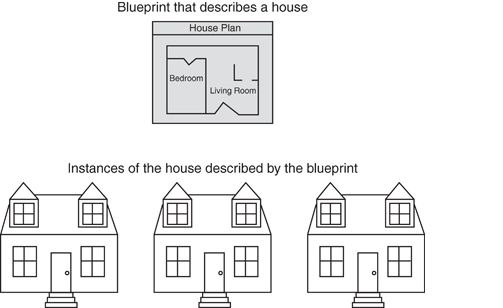
\includegraphics[scale=0.8]{Images/chapter06_BlueprintHouses.png}
    \end{figure}
\end{frame}

\begin{frame}{Classes in the Java API}
    The objects that you have used in your programs so far are created from
    classes in the Java Application Programming Interface (API).
    \\ \vspace{1em}
    The Java API consists of a set of classes included with the Java Development Environment. 
    \\ \vspace{1em}
    \begin{itemize}
        \item Each time you create a Scanner object, you are creating an instance of a class named Scanner, which is in the Java API.
        \item  When you create a Random object, you are creating an instance of a class named Random, which is in the Java API.
        \item When you need to write data to a file, you create an instance of the PrintWriter class, which is in the Java API.
    \end{itemize}
\end{frame}

\subsection{Primitive Variables vs Objects}
\begin{frame}[fragile]{Primitive Variables vs Objects}
    Recall the Java primitive data types: \textbf{byte, short, int, long, char, float, double,} and \textbf{boolean}.
    \\ \vspace{1em}
    By now you have seen many programs that use both primitive data types and objects. 
\end{frame}

\begin{frame}[fragile]{Primitive Variables vs Objects}
    The steps required to create an object differ from the steps required to create a primitive variable.
    \begin{lstlisting}
int wholeNumber;            // creating primitive variable
Random rand = new Rand();   // creating object
    \end{lstlisting}
    Primitive variables are simply storage locations in the computer’s memory. \\
    \vspace{1em}
    A variable created with a primitive data type has no built-in capabilities other than storing a value. \\
    \vspace{1em}
    When you declare a primitive variable, the compiler sets aside a chunk of memory that is big enough for that variable.
\end{frame}

\begin{frame}[fragile]{Primitive Variables vs Objects}
    Let's recall what happens "under the hood" when we declare the following in Java,
    \begin{lstlisting}
    int wholeNumber = 99;    // allocates 4 bytes of memory
    double realNumber = 123.45;  // allocates 8 bytes of memory
    \end{lstlisting}
    In a picture, we can imagine the following.
    \noindent 
    \begin{figure}[H]
    \centering
    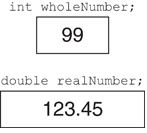
\includegraphics[scale=0.6]{Images/chapter06_NumberInBox.png}
    \end{figure}
    In a sense, dealing with primitive variables only  involves using a storage location that holds a piece of data.
\end{frame}

\begin{frame}{Primitive Variables vs Objects}
    When you are working with an object, you are typically using two things:
    \begin{enumerate}
        \item The object itself, which must be created in memory.
        \item A reference variable that refers to the object.
    \end{enumerate}

    The reference variable doesn't hold an actual piece of data that your program will work with. \\ \vspace{1em}
    It holds the object’s memory address.
    \noindent 
    \begin{figure}[H]
    \centering
    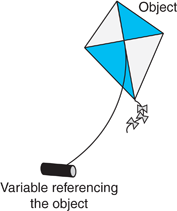
\includegraphics[scale=0.6]{Images/chapter06_ReferenceVariableAndObject.png}
    \end{figure}
\end{frame}

\begin{frame}[fragile]{Primitive Variables vs Objects}
    Let's digest the following Java statement.
    \begin{lstlisting}
Random rand = new Random();
    \end{lstlisting}
    \begin{itemize}
        \item The left hand side of the $=$ operator declares a variable named \textbf{rand}, which can be used to reference an object of the \textbf{Random} type.
        \item On the right side of the $=$ operator, the expression \textbf{new Random()} creates an object from the \textbf{Random} class, and returns that object’s memory address.
        \item  The $=$ operator assigns the memory address that was returned from the \textbf{new} operator to the \textbf{rand} variable.
    \end{itemize}
\end{frame}

\section{Writing a Class, Instance Fields and Methods, and Constructors}
\subsection{Writing a Class}
\begin{frame}{Writing a Class}
    So far we've mostly considered classes with a single \textbf{main} method. \\ \vspace{1em}
    
    We will now write a \red{class} so we can see how the terms \violet{object}, \violet{fields}, and \violet{methods} are used in practice. \\ \vspace{1em}
    
    Imagine what the \red{blueprint for a rectangle} would look like. \\ \vspace{1em} 
    
    A \violet{specific rectangle}, say, of \violet{length 10 cm and width 5 cm} is one construction inspired by the blueprint. \\ \vspace{1em}
    
    Since we are programming, it would be ideal to have functions that can \violet{adjust the length and width} for a desired rectangle.
\end{frame}

\begin{frame}{Writing a Class}
    So, our class will be called \textbf{Rectangle} with the following fields
    \begin{itemize}
        \item \textbf{length}
        \item \textbf{width}
    \end{itemize}
    and the following methods
    \begin{itemize}
        \item \textbf{setLength}
        \item \textbf{setWidth}
        \item \textbf{getLength}
        \item \textbf{getWidth}
        \item \textbf{getArea}
    \end{itemize}
    % Idea: define a "isSquare" method?
\end{frame}

\begin{frame}[fragile]{Writing a Class}
Here is an incomplete example.
    \begin{lstlisting}
public class Rectangle {
    // _private_ so fields are
    // hidden from code outside of class
    private double length = 0;
    private double width = 0;
    // _public_ so methods can be called
    // from outside of the class
    // if _static_ is not written we imply this is an
    // _instance_ method
    public void setLength(double len) {
        length = len; // updates _length_ field
        }
    }
    \end{lstlisting}
Notice we are not writing a \textbf{main} method.
\end{frame}

\begin{frame}[fragile]{Writing a Class}
We can then call the \textbf{Rectangle} class from another script:
    \begin{lstlisting}
// RectangleDemo.java in same directory as Rectangle.java
public class RectangleDemo {
    public static void main(String[] args) {
        // Make "box" variable reference a Rectangle object
        Rectangle box = new Rectangle();
        System.out.println(
            "Sending the value 10.0"
            + " to the setLength method."
            );
        box.setLength(10.0);
        System.out.println("Done.");
        }	
    }
    \end{lstlisting}
\end{frame}

\begin{frame}[fragile]{Writing a Class}
\footnotesize
Representation for initializing an instance of the Rectangle class.
    \begin{lstlisting}
Rectangle box = new Rectangle();
    \end{lstlisting}
    \noindent 
    \begin{figure}[H]
    \centering
    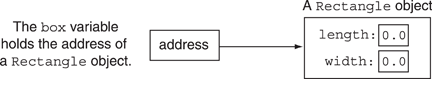
\includegraphics[scale=0.9]{Images/chapter06_InitRectangle.png}
    \end{figure}
Representation of the Rectangle object after calling the \textbf{setLength} method.
    \begin{lstlisting}
box.setLength(10.0);
    \end{lstlisting}
    \noindent 
    \begin{figure}[H]
    \centering
    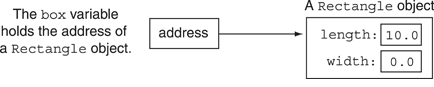
\includegraphics[scale=0.9]{Images/chapter06_ValueRectangle.png}
    \end{figure}
\end{frame}

\begin{frame}{Writing a Class}
    See the lecture video for a review on writing the entire \textbf{Rectangle} class.
\end{frame}

\begin{frame}{Accessor and Mutator Methods}
    A method that \red{gets a value} from a class’s field but does not change it is known as an \red{accessor} method (e.g., \textbf{getLength, getWidth)}. \\ \vspace{1em}
    A method that \violet{stores a value} in a field or changes the value of a field in some other way is known as a \violet{mutator} method (e.g., \textbf{setLength, setWidth}).
\end{frame}

\begin{frame}{UML Diagram}
\footnotesize
    Some people like to write a framework for a given class using a Unified Modeling Language.
    \noindent 
    \begin{figure}[H]
    \centering
    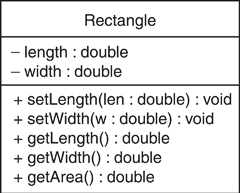
\includegraphics[scale=0.9]{Images/chapter06_ModelLanguage.png}
    \end{figure}
    Boxes from top to bottom: Class name, field names, method names. \\ \vspace{1em}
    Access specifier: negative sign for private, positive sign for public. \\ \vspace{1em} 
    Colons: Specifies output (unless it is written inside a method, which indicates input type).
\end{frame}

\subsection{Instance Fields and Methods}
\begin{frame}{Instance Fields and Methods}
    Each instance of a class has its own set of fields, which are known as instance fields. \\ \vspace{1em} 
    You can create several instances of a class and store different values in each instance’s fields. \\ \vspace{1em} 
    The methods that operate on an instance of a class are known as instance methods.
\end{frame}

\begin{frame}[fragile]{Instance Fields and Methods}
\footnotesize
    We can generate several objects derived from the same class.
    \begin{lstlisting}
Rectangle kitchen = new Rectangle();
Rectangle bedroom = new Rectangle();
Rectangle den = new Rectangle();
    \end{lstlisting}
    Which you can represent the following way.
    \noindent 
    \begin{figure}[H]
    \centering
    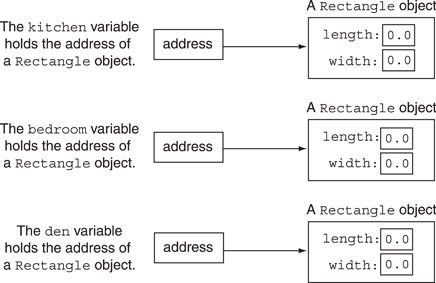
\includegraphics[scale=0.7]{Images/chapter06_RectangleInstances.png}
    \end{figure}
\end{frame}

\begin{frame}[fragile]{Instance Fields and Methods}
    We can then modify each instance's fields individually.
    \begin{lstlisting}
kitchen.setLength(10.0);
kitchen.setWidth(14.0);
bedroom.setLength(15.0);
bedroom.setWidth(12.0);
den.setLength(20.0);
den.setWidth(30.0);
    \end{lstlisting}
    And calculate the total area for the defined rooms, as an example.
\begin{lstlisting}
System.out.print(
    "The total area is "
    + (kitchen.getArea() + bedroom.getArea() + den.getArea())
    + " units squared."
    );
\end{lstlisting}
\end{frame}

\begin{frame}{Instance Fields and Methods}
    Here is the state of the objects after executing the code in the previous slide.
    \noindent 
    \begin{figure}[H]
    \centering
    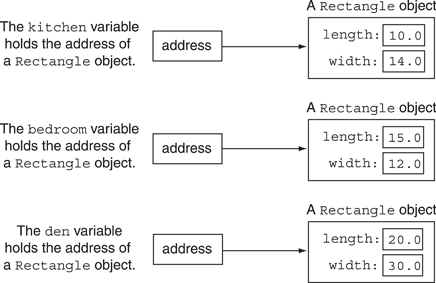
\includegraphics[scale=0.9]{Images/chapter06_RectangleInstancesWithValues.png}
    \end{figure}
\end{frame}

\subsection{Constructors}
\begin{frame}{Constructors}
    A \red{constructor} is a method that is automatically called when an \red{object is created}. \\ \vspace{1em}
    Constructors normally perform \red{initialization} or \red{setup} operations. \\ \vspace{1em}
    They are called constructors because they help construct an object.
\end{frame}

\begin{frame}[fragile]{Constructors}
    \footnotesize
    \begin{lstlisting}
public class Rectangle {
    private double length;
    private double width;
    // The folowing is the constructor.
    public Rectangle(double len, double w) {
        length = len;
        width = w;
        }
    }
    \end{lstlisting}
    Note: The constructor's header does not specify a return type. \\ \vspace{1em}
    In the next example we instantiate the object and update both instance fields in a single line.
    \begin{lstlisting}
Rectangle box = new Rectangle(7.0, 14.0);
    \end{lstlisting}
\end{frame}

\begin{frame}[fragile]{Constructors}
    If you do not explicitly write a constructor, Java provides a default constructor which sets
    \begin{itemize}
        \item numeric fields default to 0
        \item \textbf{boolean} fields default to \textbf{false}
        \item any reference variable defaults to \textbf{null}        
    \end{itemize}
    \begin{lstlisting}
// If using default constructor
Rectangle rectObj = new Rectangle(); // Perfectly fine

// If explicitly writing a constructor
Rectangle rectObj = new Rectangle(); // Error
    \end{lstlisting}
\end{frame}

\section{Objects as Arguments, Overloading, Package and Import}
\subsection{Objects as Arguments}
\begin{frame}{Objects as Arguments}
What if we want to have objects be input to methods? \\ \vspace{1em}
We can pass the object’s address into the method’s parameter variable. \\ \vspace{1em}
As a result, the parameter references the object. \\ \vspace{1em}

See lecture video for a demo using the Die.java and DieArgument.java programs.
\end{frame}

\subsection{Overloading Methods and Constructors}
\begin{frame}[fragile]{Overloading Methods and Constructors}
\footnotesize
Two or more methods in a class may have the same name as long as their parameter lists are different. \\ \vspace{1em} 
This also applies to constructors. \\ \vspace{1em}
When a method is overloaded, it means that multiple methods in the same class have the same name, but use different types of parameters. \\
\vspace{1em}
    \begin{lstlisting}
public int add(int num1, int num2) {
    int sum = num1 + num2;
    return sum;
    }
public String add(String str1, String str2) {
    String combined = str1 + str2;
    return combined;
    }
    \end{lstlisting}
\end{frame}

\begin{frame}[fragile]{Overloading Methods and Constructors}
    Matching a method call with the correct method is known as binding. \\ \vspace{1em}
    Java uses a method’s signature to distinguish it from other methods of the same name. \\ \vspace{1em}
    A method’s signature consists of the method’s name and the data types of the method’s parameters, in the order that they appear. \\ \vspace{1em}
    The method’s return type is not part of the signature. 
\end{frame}

\begin{frame}[fragile]{Overloading Methods and Constructors}
Constructors can also be overloaded.
    \begin{lstlisting}
public Rectangle() {
    length = 0.0;
    width = 0.0;
    }
public Rectangle(double len, double w) {
    length = len;
    width = w;
    }
    \end{lstlisting}
    Hence, both of the following statements are valid.
    \begin{lstlisting}
Rectangle box1 = new Rectangle();
Rectangle box2 = new Rectangle(5.0, 10.0);
    \end{lstlisting}
\end{frame}

\begin{frame}{Scope and Instance Fields}
    Instance fields are visible to all of the class’s instance methods. \\ \vspace{1em}
    An instance field can be accessed by any instance method in the same class as the field. \\ \vspace{1em}
    If an instance field is declared with the public access specifier, it can also be accessed by code outside the class.
\end{frame}

\subsection{Packages and Import Statements}
\begin{frame}{Packages and Import Statements}
    The classes in the Java API are organized into packages. \\ \vspace{1em}
    An import statement tells the compiler which package a class is located in. \\ \vspace{1em} 
    You've already used a few classes from the API, such as the \textbf{String} class, the \textbf{Scanner} class, the \textbf{JOptionPane} class, and the \textbf{Random} class. 
\end{frame}

\begin{frame}[fragile]{Packages and Import Statements}
    All of the classes in the Java API are organized into packages. \\ \vspace{1em} 
    A package is simply a group of related classes. \\ \vspace{1em} 
    Each package also has a name. \\ \vspace{1em} 
    For example, the \textbf{Scanner} class is in the \textbf{java.util} package.
        \begin{lstlisting}
// Tell the compiler that Scanner class is in
// the java.util package
import java.util.Scanner;
        \end{lstlisting}
\end{frame}

\begin{frame}[fragile]{Packages and Import Statements}
    There are two types of import statements: explicit and wildcard.
    \begin{itemize}
        \item Explicit
        \begin{lstlisting}
import java.util.Scanner;
import java.util.Random;            
        \end{lstlisting}
        \item Wildcard
        \begin{lstlisting}
import java.util.*; // Import all classes in package            
        \end{lstlisting}
    \end{itemize}
Note: The \textbf{java.lang} package is imported automatically imported into every Java program.
\end{frame}

% \begin{frame}{Writing a Class}
%     _Example of calling Rectangle class from a different class.
% \end{frame}

% \begin{frame}{Writing a Class}
%     _Show full program.
% \end{frame}

% \begin{frame}{Writing a Class}
%     _Example of defining different instances for kitchen, den, and bedroom.
% \end{frame}

% \begin{frame}{Writing a Class}
%     _Constructors
% \end{frame}

\end{document}

